\documentclass[12pt, twoside]{article}
\usepackage[letterpaper, margin=1in, headsep=0.5in]{geometry}
\usepackage[english]{babel}
\usepackage[utf8]{inputenc}
\usepackage{amsmath}
\usepackage{amsfonts}
\usepackage{amssymb}
\usepackage{tikz}
\usetikzlibrary{quotes, angles}
\usepackage{graphicx}
%\usepackage{pgfplots}
%\pgfplotsset{width=10cm,compat=1.9}
%\usepgfplotslibrary{statistics}
%\usepackage{pgfplotstable}
%\usepackage{tkz-fct}
%\usepackage{venndiagram}

\usepackage{fancyhdr}
\pagestyle{fancy}
\fancyhf{}

\fancyhead[LE]{\thepage}
\fancyhead[RO]{\thepage \\ Name: \hspace{4cm} \, \\}
\fancyhead[LO]{BECA / Dr. Huson / Geometry 10th Grade\\* Unit 5: Transformation, dilation, \& scale \\ 6 November 2019}

\renewcommand{\headrulewidth}{0pt}

\begin{document}
\subsubsection*{5.2 Do Now: Dilating a triangle, calculating lengths}
  \begin{enumerate}

  \item A dilation centered at $A$ with $k=3$ maps $\triangle ABC \rightarrow \triangle A'B'C'$. Given the sides of the preimage, $AC = 8.5$, $BC = 6.25$, and $AB = 10.5$, find the corresponding lengths of the image, writing your answer showing the multiplication by the value of $k$ using proper notation.
    \vspace{1cm}
    \begin{flushright}
    \begin{tikzpicture}[scale=0.8]
      \draw [-, thick] (0,0) node[above left]{$A'$}--
      (10,0) node[below]{$C'$}--
      (10,7.5) node[above left]{$B'$}--cycle;
      \draw [thick] (4,0)--(4,3);
      \draw [fill] (0,0) circle [radius=0.05] node[below left]{$A$};
      \draw [fill] (4,0) circle [radius=0.05] node[below]{$C$};
      \draw [fill] (4,3) circle [radius=0.05] node[above left]{$B$};
      \node at (2, 0) [below]{$8.5$};
      \node at (2, 2) [above]{$10.5$};
      \node at (4, 1.5) [right]{$6.25$};
    \end{tikzpicture}
  \end{flushright} 

  \item A dilation centered at $A$ maps $\triangle ABC \rightarrow \triangle A'B'C'$. Given the sides of the preimage, $AC = 4$, $BC = 3$, $AB = 5$, and of $B'C' = 7.5$ find the scale factor $k$ and the lengths $A'C'$ and $A'B'$.\\[0.5cm]
  Spicy: Find $CC'$.
    \vspace{1cm}
    \begin{flushright}
    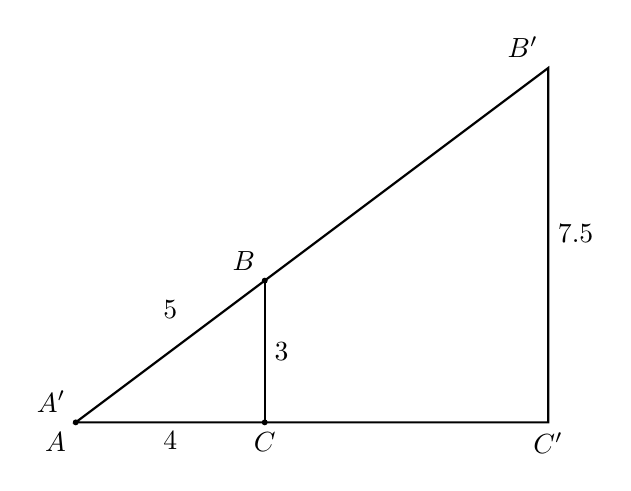
\begin{tikzpicture}[scale=0.6]
      \draw [-, thick] (0,0) node[above left]{$A'$}--
      (10,0) node[below]{$C'$}--
      (10,7.5) node[above left]{$B'$}--cycle;
      \draw [thick] (4,0)--(4,3);
      \draw [fill] (0,0) circle [radius=0.05] node[below left]{$A$};
      \draw [fill] (4,0) circle [radius=0.05] node[below]{$C$};
      \draw [fill] (4,3) circle [radius=0.05] node[above left]{$B$};
      \node at (2, 0) [below]{$4$};
      \node at (2, 2) [above]{$5$};
      \node at (10, 4) [right]{$7.5$};
      \node at (4, 1.5) [right]{$3$};
    \end{tikzpicture}
  \end{flushright} 

\end{enumerate}
\end{document}
